\section*{4/27}
  $f_i = P($ ever reenter $i | X_0 = i)$\\
  The state $i$ is \underline{recurrent} if $f_i = 1$.\\
  The state $i$ is \underline{transient} if $f_i < 1$.\\
  $P($ visit $i$ $n$ times $| X_0 = i) = f_i^{n-1}(1 - f_i)$\\
  $$
    E(\text{number of visits to } i | X_0 = i) = \frac{1}{1 - f_i}
  $$
  $$
    E(\text{number of visits to } i | X_0 = i) = E(\sum_{n = 0}^{\infty} I_n | X_0 = i)
  $$
  where $I_n = I\{X_n = i\}$, $n = 0, 1, 2, \ldots$\\
  \begin{eqnarray*}
    I_n & = & \sum_{n = 0}^{\infty}P(X_n = i | X_0 = i)\\
      & = & \sum_{n = 0}^{\infty}P_{ii}^n\\
  \end{eqnarray*}
  \begin{theorem}
    1 is recurrent $\Leftrightarrow$  $\sum_{n = 1}^{\infty}P_{ii}^n = \infty$
  \end{theorem}
  If a Markov chain only has finitely many states, then there must be at 
  least one recurrent state. Why?\\
  If all states are transient, then all the states will be visited only finitely
  many times. That is impossible. \\
  \begin{proposition}
    If $i$ is recurrent, and $i \leftrightarrow$ j, then also, $j$ is recurrent.
    If the chain is irreducible, then either all states are recurrent or all
    transient.
  \end{proposition}
  \begin{proof}
    $P_{ij}^k > 0, P_{ji}^m > 0$ for some $k,m$.\\
    For any $n \ge 0$:
    $$
      P_{ij}^{m + n + k} \ge P_{ji}^m P_{ii}^n P_{ij}^k
    $$
    If a state is recurrent, then $f_i = 1$. \\
    Then, $E(\text{number of visits to } i | X_0 = i) = \frac{1}{1 - f_i} = \infty$.\\
    If $\sum_{n = 0}^{\infty} P_{ii} = \infty$, then 
    $\sum_{n = 0}^{\infty} P_{jj}^{m+n+k}=\infty$, so
    $\sum_{l = 0}^{\infty} P_{jj}^{l} = \infty$.\\
    If $i$ is recurrent, then so is $j$.
  \end{proof}

  \noindent\underline{Example}:
  $$
    P = \left[
      \begin{array}{c c c c}
        0 & 0 & \frac{1}{2} & \frac{1}{2}\\
        1 & 0 & 0 & 0\\
        0 & 1 & 0 & 0\\
        0 & 1 & 0 & 0\\
      \end{array}
      \right]
  $$
  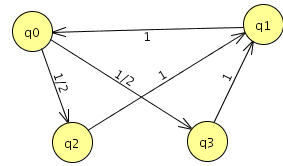
\includegraphics{Ex1_4_27.png}\\
  As we can see every element can reach each other, so the chain is 
  irreducible. We can also see that state 0 whether it chooses to
  go to state 2 and 3 will end up at state 1 and back to state 0.
  Therefore, it is recurrent and the entire thing is also recurrent.\\

  \noindent\underline{Example}:
    $$
      P = \left[
        \begin{array}{c c c c c c}
          0 & 1 & 0 & 0 & 0 & 0\\
          4 & 6 & 0 & 0 & 0 & 0\\
          3 & 0 & 4 & 2 & 1 & 0\\
          0 & 0 & 0 & 3 & 7 & 0\\
          0 & 0 & 0 & 5 & 0 & 5\\
          0 & 0 & 0 & 3 & 0 & 2\\
        \end{array}
      \right]
    $$
    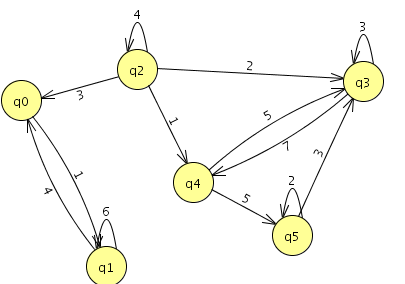
\includegraphics{Ex2_4_27.png}\\
    As we can see, nothing can reach 2 besides 2 itself. Therefore, 2 is
    in a group of its own. 0 and 1 can reach other and nothing else, so it
    is in a group of its own. 3, 4, and 5 can reach each other.\\
    As we can see, 2 can only reach itself sometimes. Therefore, $j_2 < 1$ 
    making it transient.\\
    When we are at state 1 and choose to go to 0, it will always come back to 1.
    Also, state 1 can choose to stay. Therefore, $j_1 = 1$, which then
    means that $j_0 = 1$ making both of them recurrent.\\
    We can also see that $\{3, 4, 5\}$ is recurrent.\\

  \noindent\underline{Example}:
    Simple random walk on $\mathbb{Z}$. When $p = \frac{1}{2}$, this is
    a simple symmetric random walk.\\
    Simple random walk on $\mathbb{Z}^2$.\\
    Simple random walk on $\mathbb{Z}^3$.\\
    Higher dimensions makes for lower probability to return to origin.\\
    In the 1 dimension case, 
    $$
      P_{00}^{2n - 1} = 0 \text{ (because if you walk out $n$ steps, 
        you need to walk back $n$ steps)}
    $$
    $$
      P_{00}^{2n} = \binom{2n}{n}p^n(1 - p)^n \text{($n$ steps to the 
        left and $n$ steps to the right. Pick $n$ steps out of $2n$ 
        steps to be left.)}
    $$
    Stirling's formula:
    $$
      n! \approx n^ne^{-n} \sqrt{2\pi n}
    $$
    So, according to Stirling's formula,
    \begin{eqnarray*}
      \binom{2n}{n} & = & \frac{(2n)!}{(n!)^2}\\
        & = & \frac{(2n)^{2n}e^{-2n}\sqrt{2\pi2n}}{n^{2n} e^{-2n} 2\pi n}\\
        & = & \frac{2^{2n}}{n\pi}
    \end{eqnarray*}


